\documentclass[letterpaper]{article}
% FinFM @ AAAI-27, short paper (benchmark track, non-archival): up to 4 pages of technical
% content, unlimited references and appendices. Official AAAI-27 style, anonymous
% submission. The lines marked "fixed" come from the author kit and must stay as they are.
% Numbers, figures and tables are read from ../latex_acl2027, so this version, the 7-page
% version in ../finfm_aaai27 and the ACL 2027 draft cannot drift apart; the condensed text
% is in sections/.
\usepackage[submission]{aaai2027}
\usepackage[hyphens]{url} % fixed
\usepackage{graphicx} % fixed
\urlstyle{rm} % fixed
\def\UrlFont{\rm} % fixed
\usepackage{natbib} % fixed, without options
\usepackage{caption} % fixed, without options
\frenchspacing % fixed
\setlength{\pdfpagewidth}{8.5in} % fixed
\setlength{\pdfpageheight}{11in} % fixed
\usepackage{amsmath,amssymb,booktabs,array,listings}
\usepackage{tikz}
\usetikzlibrary{arrows.meta,positioning,fit,backgrounds,calc,shadows,shapes.geometric,3d,shadows.blur,fadings,shadings}
\definecolor{finblue}{HTML}{2A78D6}
\definecolor{finorange}{HTML}{EB6834}
\definecolor{fingray}{HTML}{52514E}
\definecolor{finaqua}{HTML}{1BAF7A}
\definecolor{finmagenta}{HTML}{C2408B}
% Small pictograms for the figures, drawn in TikZ (no icon font needed). Use as
% \pic[draw=white, line width=0.55pt] at (x,y) {fin doc}; size about 0.3 cm.
\tikzset{
  fin doc/.pic={
    \draw[pic actions, fill=none, line join=round] (-0.10,-0.14) -- (-0.10,0.14) -- (0.04,0.14)
      -- (0.10,0.08) -- (0.10,-0.14) -- cycle;
    \draw[pic actions, fill=none] (0.04,0.14) -- (0.04,0.08) -- (0.10,0.08);
    \draw[pic actions, fill=none, line width=0.4pt] (-0.055,0.03) -- (0.055,0.03)
      (-0.055,-0.025) -- (0.055,-0.025) (-0.055,-0.08) -- (0.03,-0.08);},
  fin check/.pic={
    \draw[pic actions, fill=none] (0,0) circle (0.13);
    \draw[pic actions, fill=none, line width=0.75pt, line cap=round, line join=round]
      (-0.065,0.0) -- (-0.018,-0.05) -- (0.07,0.055);},
  fin loop/.pic={
    \draw[pic actions, fill=none, line width=0.7pt, -{Stealth[length=2.4pt, width=2.8pt]}]
      (0.13,0.0) arc[start angle=0, end angle=285, radius=0.12];},
  fin plug/.pic={
    \draw[pic actions, fill=none, rounded corners=0.6pt] (-0.09,-0.02) rectangle (0.09,0.07);
    \draw[pic actions, fill=none, line cap=round] (-0.045,0.07) -- (-0.045,0.14) (0.045,0.07) -- (0.045,0.14);
    \draw[pic actions, fill=none, line cap=round] (0,-0.02) -- (0,-0.14);},
  fin robot/.pic={
    \draw[pic actions, fill=none, rounded corners=1pt] (-0.12,-0.10) rectangle (0.12,0.08);
    \fill[pic actions, draw=none] (-0.05,-0.005) circle (0.022) (0.05,-0.005) circle (0.022);
    \draw[pic actions, fill=none, line cap=round] (0,0.08) -- (0,0.13);
    \fill[pic actions, draw=none] (0,0.145) circle (0.022);},
  fin gauge/.pic={
    \draw[pic actions, fill=none] (-0.13,-0.05) arc[start angle=180, end angle=0, radius=0.13];
    \draw[pic actions, fill=none, line width=0.7pt, line cap=round] (0,-0.05) -- (0.07,0.04);
    \fill[pic actions, draw=none] (0,-0.05) circle (0.025);},
  fin lock/.pic={
    \draw[pic actions, fill=none, rounded corners=0.8pt] (-0.10,-0.13) rectangle (0.10,0.02);
    \draw[pic actions, fill=none] (-0.06,0.02) -- (-0.06,0.07) arc[start angle=180, end angle=0,
      radius=0.06] -- (0.06,0.02);
    \fill[pic actions, draw=none] (0,-0.055) circle (0.022);},
  fin chart/.pic={
    \fill[pic actions, draw=none] (-0.11,-0.12) rectangle (-0.05,-0.02)
      (-0.03,-0.12) rectangle (0.03,0.06) (0.05,-0.12) rectangle (0.11,0.12);},
  fin code/.pic={
    \draw[pic actions, fill=none, line cap=round, line join=round, line width=0.65pt]
      (-0.06,0.08) -- (-0.13,0) -- (-0.06,-0.08) (0.06,0.08) -- (0.13,0) -- (0.06,-0.08);
    \draw[pic actions, fill=none, line cap=round, line width=0.5pt] (0.025,0.11) -- (-0.025,-0.11);},
  fin search/.pic={
    \draw[pic actions, fill=none, line width=0.6pt] (-0.025,0.035) circle (0.085);
    \draw[pic actions, fill=none, line width=0.9pt, line cap=round] (0.04,-0.03) -- (0.11,-0.11);},
  fin feed/.pic={
    \fill[pic actions, draw=none] (-0.085,-0.085) circle (0.028);
    \draw[pic actions, fill=none, line width=0.6pt, line cap=round]
      (-0.085,0.005) arc[start angle=90, end angle=0, radius=0.09]
      (-0.085,0.075) arc[start angle=90, end angle=0, radius=0.16];},
  fin link/.pic={
    \draw[pic actions, fill=none, line width=0.6pt, rounded corners=1.6pt, rotate=45]
      (-0.13,-0.04) rectangle (0.0,0.04) (-0.0,-0.04) rectangle (0.13,0.04);},
  fin sigma/.pic={
    \draw[pic actions, fill=none, line width=0.7pt, line cap=round, line join=round]
      (0.085,0.11) -- (-0.085,0.11) -- (0.02,0.0) -- (-0.085,-0.11) -- (0.085,-0.11);},
  fin db/.pic={
    \draw[pic actions, fill=none, line width=0.6pt] (0,0.085) ellipse (0.1 and 0.035);
    \draw[pic actions, fill=none, line width=0.6pt] (-0.1,0.085) -- (-0.1,-0.085)
      arc[start angle=180, end angle=360, x radius=0.1, y radius=0.035] -- (0.1,0.085);
    \draw[pic actions, fill=none, line width=0.5pt] (-0.1,0.0)
      arc[start angle=180, end angle=360, x radius=0.1, y radius=0.035];},
  fin braces/.pic={
    \draw[pic actions, fill=none, line width=0.65pt, rounded corners=0.9pt, line cap=round]
      (-0.025,0.12) -- (-0.065,0.12) -- (-0.065,0.03) -- (-0.115,0) -- (-0.065,-0.03)
      -- (-0.065,-0.12) -- (-0.025,-0.12)
      (0.025,0.12) -- (0.065,0.12) -- (0.065,0.03) -- (0.115,0) -- (0.065,-0.03)
      -- (0.065,-0.12) -- (0.025,-0.12);},
  fin term/.pic={
    \draw[pic actions, fill=none, line width=0.55pt, rounded corners=1pt]
      (-0.13,-0.1) rectangle (0.13,0.1);
    \draw[pic actions, fill=none, line width=0.65pt, line cap=round, line join=round]
      (-0.075,0.035) -- (-0.03,0.0) -- (-0.075,-0.035);
    \draw[pic actions, fill=none, line width=0.65pt, line cap=round] (0.0,-0.045) -- (0.07,-0.045);},
  fin person/.pic={
    \fill[pic actions, draw=none] (0,0.055) circle (0.052);
    \fill[pic actions, draw=none] (-0.11,-0.125) arc[start angle=180, end angle=0, radius=0.11]
      -- cycle;},
}

% Generated by make_numbers.py from the library; do not edit by hand.
\newcommand{\NSkills}{131}
\newcommand{\NPlugins}{17}
\newcommand{\NReferenceFiles}{75}
\newcommand{\NScripts}{125}
\newcommand{\NListingTokens}{27,700}
\newcommand{\NFederatedPacks}{92}
\newcommand{\NFederatedSkills}{2,390}
\newcommand{\NLensPacks}{3}
\newcommand{\NLensSkills}{100}
\newcommand{\NKOLProfiles}{40}
\newcommand{\NAlgorithms}{48}
\newcommand{\NAlgorithmTasks}{11}
\newcommand{\NNative}{25}
\newcommand{\NAdapters}{23}
\newcommand{\NOptionalLibraries}{13}
\newcommand{\NGuards}{39}
\newcommand{\NGuardsExported}{32}
\newcommand{\NGuardsPythonOnly}{7}
\newcommand{\NTools}{67}
\newcommand{\NCards}{6}
\newcommand{\NCardFamilies}{3}
\newcommand{\NCauses}{5}
\newcommand{\NMethods}{7}
\newcommand{\NArms}{4}
\newcommand{\NTasks}{34}
\newcommand{\NTaskAlgorithms}{17}
\newcommand{\NDevTasks}{18}
\newcommand{\NDevAlgorithms}{9}
\newcommand{\NHeldTasks}{16}
\newcommand{\NHeldAlgorithms}{8}
\newcommand{\NHeldFamilies}{5}
\newcommand{\NFamilies}{5}
\newcommand{\NSeeds}{3}
\newcommand{\NRows}{128}
\newcommand{\NRowsEFour}{96}
\newcommand{\NEFourTasks}{4}
\newcommand{\NForcedDev}{5}
\newcommand{\NDrawn}{12}
\newcommand{\NDrawnDev}{4}
\newcommand{\NModels}{5}
\newcommand{\NMainEpisodes}{3,360}
\newcommand{\NAblationEpisodes}{1,440}
\newcommand{\NRealEpisodes}{1,120}
\newcommand{\NRealRows}{128}
\newcommand{\NRealSplitRow}{45}
\newcommand{\RealFirst}{31 March 2022}
\newcommand{\RealLast}{3 October 2022}
\newcommand{\RefGapMinVariance}{1.4\times10^{-6}}
\newcommand{\RefGapOther}{2.8\times10^{-14}}
\newcommand{\BudgetAttempts}{3}
\newcommand{\BudgetCalls}{6}
\newcommand{\BudgetTokens}{12,000}
\newcommand{\FitEpisodes}{48}
\newcommand{\FitProposals}{6}
\newcommand{\FitCalls}{600}
\newcommand{\FitTokens}{1,200,000}
\newcommand{\EvolveGenerations}{3}
\newcommand{\EvolveMinibatch}{4}

\graphicspath{{../latex_acl2027/}}
\makeatletter\def\input@path{{../latex_acl2027/}}\makeatother % shared tables
\lstset{basicstyle=\ttfamily\footnotesize,columns=fullflexible,keepspaces=true,
        showstringspaces=false,frame=none,xleftmargin=0pt}
\newcommand{\pending}[1]{{\color{red}[#1]}}
\providecommand{\href}[2]{#2} % aaai2027.bst emits \href; AAAI forbids hyperref
\newcommand{\lib}{\textsc{Fin-RSI}}
\setcounter{secnumdepth}{2}

\title{\lib{}: An Agent-Native Library of Financial Skills, Checks, and Self-Improvement}
\author{Anonymous submission}
\affiliations{}

\begin{document}
\maketitle

\begin{abstract}
Financial research code fails silently: a program that applies stock splits twice, or
trades on the closing price it reads, still runs and still returns a backtest. We present
\lib{}, an agent-native Python library that puts three things behind interfaces a
language-model agent can call: \emph{skills} (\NSkills{} dated skill documents,
\NAlgorithms{} algorithms and \NCards{} rule cards), \emph{checks} (\NGuards{} guards,
including property checks that need no expected output) and \emph{self-improvement}
(\NMethods{} methods behind one \texttt{fit}/\texttt{solve}/\texttt{state} interface with
metered, equal budgets). With it comes a suite of \NTasks{} financial programming tasks on
synthetic and real prices, each with an independent reference and a hidden grader that no
method sees. \pending{One sentence of results.} The library, tasks and protocol will be
released.

\end{abstract}

\begin{figure*}[t]
\centering
% Figure 1: the library at a glance. Information comes in on the left, an agent is composed in
% the middle (the user's model, one self-improvement method, any checks, skills and investor
% templates) and the library is used from the right. Badges and labels are counts from the code
% on 2026-11-05: macros from numbers.tex where one exists, otherwise noted here (8 adapters,
% 4 discovery sources, 9 collectors in fin_skills.data and fin_skills.collect; 14 bridged
% libraries in fin_skills.bridges). Needs the TikZ libraries 3d, shadows.blur, fadings, shadings.
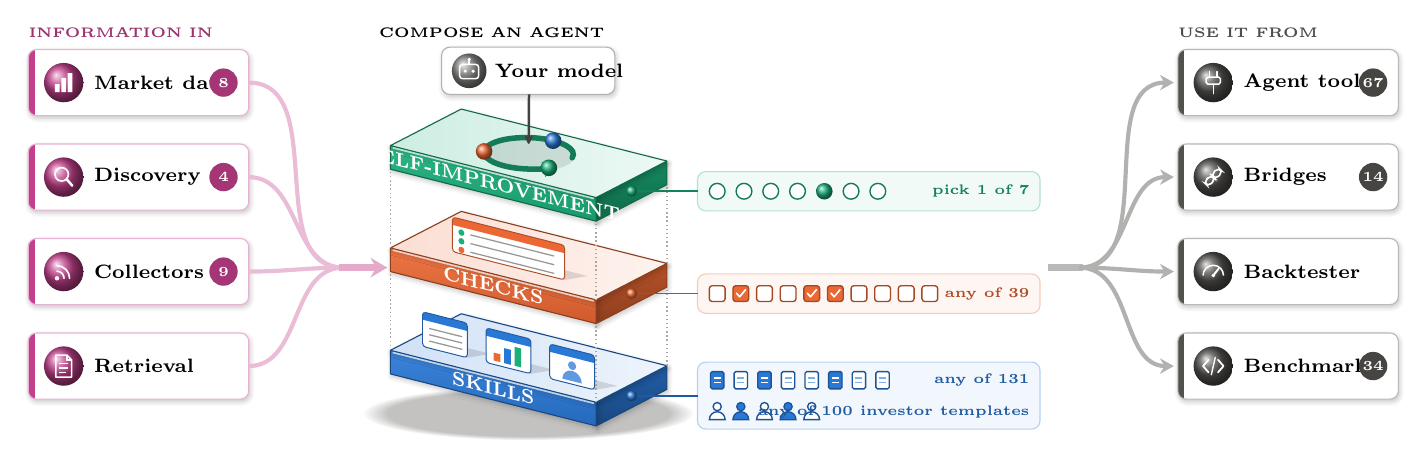
\begin{tikzpicture}[
  font=\scriptsize,
  >={Stealth[length=4pt, width=3.8pt, round]},
  head/.style={font=\tiny\bfseries, anchor=south west, inner sep=0pt},
  ball/.style={circle, shading=ball, ball color=#1, inner sep=0pt, minimum size=9pt},
  ball/.default=finblue,
  iso/.style={x={(0.95cm,-0.24cm)}, y={(0.62cm,0.32cm)}, z={(0cm,1cm)}},
  shade/.style={blur shadow={shadow blur steps=6, shadow xshift=0.45pt, shadow yshift=-0.9pt,
                             shadow opacity=24}},
  badge/.style={circle, fill=#1, text=white, font=\tiny\bfseries, inner sep=0pt,
                minimum size=0.36cm},
  pick/.style={font=\tiny\bfseries, text=#1!75!black, anchor=east, inner sep=0pt},
]
% ================================================================== helpers
% \tile{x}{y centre}{w}{colour}{icon}{label}{badge}: a card with an accent bar, an icon and a count.
\newcommand{\tile}[7]{%
  \path[fill=white, rounded corners=3pt, shade] (#1,{#2+0.42}) rectangle ({#1+#3},{#2-0.42});
  \begin{scope}
    \clip[rounded corners=3pt] (#1,{#2+0.42}) rectangle ({#1+#3},{#2-0.42});
    \fill[#4] (#1,{#2+0.42}) rectangle ({#1+0.08},{#2-0.42});
  \end{scope}
  \draw[#4!40, rounded corners=3pt, line width=0.4pt] (#1,{#2+0.42}) rectangle ({#1+#3},{#2-0.42});
  \node[ball=#4, minimum size=0.5cm] at ({#1+0.45},#2) {};
  \pic[draw=white, fill=white, line width=0.55pt] at ({#1+0.45},#2) {#5};
  \node[anchor=west, font=\scriptsize\bfseries, inner sep=0pt] at ({#1+0.83},#2) {#6};
  \if\relax\detokenize{#7}\relax\else
    \node[badge=#4!85!black] at ({#1+#3-0.32},#2) {#7};\fi}
% \track{y bottom}{y top}{colour}: the tinted strip that holds one layer's choices.
\newcommand{\track}[3]{%
  \path[fill=#3!6, draw=#3!35, line width=0.4pt, rounded corners=3pt] (8.5,#1) rectangle (12.85,#2);}
\def\sW{2.75}\def\sD{1.45}\def\sT{0.3}\def\pitch{1.3}
% \slab{z}{colour}{label}: a shaded slab with its label printed on the front face.
\newcommand{\slab}[3]{%
  \begin{scope}[iso]
    \shade[top color=#2!78!black, bottom color=#2!60!black]
      (\sW,0,#1) -- (\sW,\sD,#1) -- (\sW,\sD,{#1+\sT}) -- (\sW,0,{#1+\sT}) -- cycle;
    \shade[top color=#2!92, bottom color=#2!88!black]
      (0,0,#1) -- (\sW,0,#1) -- (\sW,0,{#1+\sT}) -- (0,0,{#1+\sT}) -- cycle;
    \shade[left color=#2!22, right color=#2!8]
      (0,0,{#1+\sT}) -- (\sW,0,{#1+\sT}) -- (\sW,\sD,{#1+\sT}) -- (0,\sD,{#1+\sT}) -- cycle;
    \draw[#2!60!black, line width=0.4pt, line join=round]
      (0,0,#1) -- (\sW,0,#1) -- (\sW,\sD,#1) -- (\sW,\sD,{#1+\sT}) -- (0,\sD,{#1+\sT})
      -- (0,0,{#1+\sT}) -- cycle (0,0,{#1+\sT}) -- (\sW,0,{#1+\sT}) -- (\sW,\sD,{#1+\sT})
      (\sW,0,{#1+\sT}) -- (\sW,0,#1);
    \draw[white, opacity=0.7, line width=0.6pt] (0.03,0,{#1+\sT-0.02}) -- (\sW-0.03,0,{#1+\sT-0.02});
    \begin{scope}[canvas is xz plane at y=0]
      \node[transform shape, text=white, font=\scriptsize\bfseries] at (\sW/2, {#1+\sT/2}) {#3};
    \end{scope}
  \end{scope}}
% \stand{x}{y}{z}{w}{h}{colour}{content}: a card standing on a top face, shadow cast behind.
\newcommand{\stand}[7]{%
  \begin{scope}[iso]
    \begin{scope}[canvas is xy plane at z=#3]
      \fill[black, opacity=0.12] (#1, #2) -- ({#1+#4}, #2) -- ({#1+#4+0.14}, {#2+0.26})
        -- ({#1+0.14}, {#2+0.26}) -- cycle;
    \end{scope}
    \begin{scope}[canvas is xz plane at y=#2, shift={(#1, #3)}]
      \fill[white, rounded corners=1.2pt] (0,0) rectangle (#4, #5);
      \begin{scope}
        \clip[rounded corners=1.2pt] (0,0) rectangle (#4, #5);
        \fill[#6] (0, #5-0.1) rectangle (#4, #5);
      \end{scope}
      \draw[#6!75!black, line width=0.35pt, rounded corners=1.2pt] (0,0) rectangle (#4, #5);
      #7
    \end{scope}
  \end{scope}}

% ================================================================== left: information in
\node[head, text=finmagenta!80!black] at (0, 5.22) {INFORMATION IN};
\tile{0}{4.65}{2.8}{finmagenta}{fin chart}{Market data}{8}
\tile{0}{3.45}{2.8}{finmagenta}{fin search}{Discovery}{4}
\tile{0}{2.25}{2.8}{finmagenta}{fin feed}{Collectors}{9}
\tile{0}{1.05}{2.8}{finmagenta}{fin doc}{Retrieval}{}
\foreach \y in {4.65, 3.45, 2.25, 1.05}
  \draw[line width=1.5pt, finmagenta!35] (2.8, \y) to[out=0, in=180] (4.0, 2.3);
\draw[-{Stealth[length=6pt, width=7pt]}, line width=2.4pt, finmagenta!45] (3.95, 2.3) -- (4.56, 2.3);

% ================================================================== middle: compose an agent
\node[head] at (4.45, 5.22) {COMPOSE AN AGENT};
\begin{scope}[shift={(4.6, 0.95)}]
\fill[fingray, opacity=0.35, path fading=circle with fuzzy edge 15 percent]
  (1.75, -0.5) ellipse (2.1cm and 0.34cm);
\slab{0}{finblue}{SKILLS}
\stand{0.22}{0.32}{\sT}{0.6}{0.44}{finblue}{%
  \foreach \yy in {0.25, 0.17, 0.09} \draw[fingray!60, line width=0.45pt] (0.09,\yy) -- (0.53,\yy);}
\stand{1.07}{0.32}{\sT}{0.6}{0.44}{finblue}{%
  \fill[finorange] (0.1,0.05) rectangle (0.19,0.15); \fill[finblue] (0.24,0.05) rectangle (0.33,0.24);
  \fill[finaqua] (0.38,0.05) rectangle (0.47,0.29);}
\stand{1.92}{0.32}{\sT}{0.6}{0.44}{finblue}{%
  \fill[finblue!75] (0.3,0.235) circle (0.055);
  \fill[finblue!75] (0.17,0.04) arc[start angle=180, end angle=0, radius=0.13] -- cycle;}
\slab{\pitch}{finorange}{CHECKS}
\stand{0.62}{0.32}{{\pitch+\sT}}{1.5}{0.44}{finorange}{%
  \foreach \yy/\c in {0.27/finaqua, 0.16/finaqua, 0.05/finorange} {
    \fill[\c] (0.12,\yy) circle (0.04); \draw[fingray!60, line width=0.45pt] (0.24,\yy) -- (1.36,\yy);}}
\slab{2*\pitch}{finaqua}{SELF-IMPROVEMENT}
\begin{scope}[iso]
  \begin{scope}[canvas is xy plane at z={2*\pitch+\sT}]
    \fill[black, opacity=0.1] (\sW/2+0.05, \sD/2-0.06) circle (0.5);
    \draw[finaqua!70!black, line width=2pt, line cap=round, -{Stealth[length=4.5pt, width=5.5pt]}]
      ({\sW/2+0.5*cos(20)}, {\sD/2+0.5*sin(20)}) arc[start angle=20, end angle=340, radius=0.5];
  \end{scope}
  \foreach \a/\c in {90/finblue, 210/finorange, 330/finaqua}
    \node[ball=\c, minimum size=6pt] at ({\sW/2+0.5*cos(\a)}, {\sD/2+0.5*sin(\a)}, {2*\pitch+\sT}) {};
  \foreach \u/\v in {0/0, \sW/0, \sW/\sD}
    \draw[fingray!50, densely dotted, line width=0.5pt]
      (\u, \v, \sT) -- (\u, \v, \pitch) (\u, \v, {\pitch+\sT}) -- (\u, \v, {2*\pitch});
  \foreach \k in {0, 1, 2} \coordinate (r\k) at (\sW, \sD/2, {\k*\pitch+\sT/2});
  \coordinate (topc) at (\sW/2, \sD/2, {2*\pitch+\sT});
\end{scope}
\end{scope}

% the user's model drives the stack
\path[fill=white, rounded corners=3pt, shade] (5.25, 5.1) rectangle (7.45, 4.5);
\draw[fingray!45, rounded corners=3pt, line width=0.4pt] (5.25, 5.1) rectangle (7.45, 4.5);
\node[ball=fingray!70, minimum size=0.44cm] (rob) at (5.6, 4.8) {};
\pic[draw=white, fill=white, line width=0.55pt] at (rob) {fin robot};
\node[anchor=west, font=\scriptsize\bfseries, inner sep=0pt] at (5.92, 4.8) {Your model};
\draw[->, line width=0.9pt, fingray!80!black] (6.36, 4.5) -- ($(topc) + (0, 0.12)$);

% each layer's choices: filled marks are one agent
\track{3.02}{3.52}{finaqua}
\track{1.72}{2.22}{finorange}
\track{0.25}{1.1}{finblue}
\foreach \k/\col in {0/finblue, 1/finorange, 2/finaqua} {
  \draw[\col!75!black, line width=0.5pt] (r\k) -- (r\k -| 8.5, 0);
  \node[ball=\col, minimum size=4pt] at (r\k) {};}
% self-improvement: pick one (radio)
\foreach \i in {0,...,6} {
  \ifnum\i=4 \node[ball=finaqua, minimum size=0.21cm] at ({8.75+0.34*\i}, 3.27) {};
  \else \draw[finaqua!70!black, fill=white, line width=0.5pt] ({8.75+0.34*\i}, 3.27) circle (0.1);\fi}
\node[pick=finaqua] at (12.72, 3.27) {pick 1 of \NMethods{}};
% checks: pick any (boxes)
\foreach \i in {0,...,9} {
  \def\cx{8.75+0.3*\i}
  \ifnum\i=1 \def\on{1}\else\ifnum\i=4 \def\on{1}\else\ifnum\i=5 \def\on{1}\else\def\on{0}\fi\fi\fi
  \ifnum\on=1
    \draw[finorange!70!black, fill=finorange, line width=0.5pt, rounded corners=1pt]
      ({\cx-0.1}, 1.87) rectangle ({\cx+0.1}, 2.07);
    \draw[white, line width=0.6pt, line cap=round, line join=round]
      ({\cx-0.055}, 1.975) -- ({\cx-0.015}, 1.93) -- ({\cx+0.06}, 2.02);
  \else
    \draw[finorange!70!black, fill=white, line width=0.5pt, rounded corners=1pt]
      ({\cx-0.1}, 1.87) rectangle ({\cx+0.1}, 2.07);\fi}
\node[pick=finorange] at (12.72, 1.97) {any of \NGuards{}};
% skills: pick any (documents) and investor templates (people)
\foreach \i in {0,...,7} {
  \def\cx{8.75+0.3*\i}
  \ifnum\i=0 \def\on{1}\else\ifnum\i=2 \def\on{1}\else\ifnum\i=5 \def\on{1}\else\def\on{0}\fi\fi\fi
  \ifnum\on=1 \def\fc{finblue}\def\lc{white}\else \def\fc{white}\def\lc{finblue!60}\fi
  \draw[finblue!70!black, fill=\fc, line width=0.5pt, rounded corners=0.6pt]
    ({\cx-0.085}, 0.76) rectangle ({\cx+0.085}, 0.98);
  \draw[\lc, line width=0.45pt] ({\cx-0.045}, 0.90) -- ({\cx+0.045}, 0.90)
    ({\cx-0.045}, 0.84) -- ({\cx+0.045}, 0.84);}
\node[pick=finblue] at (12.72, 0.87) {any of \NSkills{}};
\foreach \i in {0,...,4} {
  \def\cx{8.75+0.3*\i}
  \ifnum\i=1 \def\fc{finblue}\else\ifnum\i=3 \def\fc{finblue}\else\def\fc{white}\fi\fi
  \draw[finblue!70!black, fill=\fc, line width=0.5pt] (\cx, 0.535) circle (0.052);
  \draw[finblue!70!black, fill=\fc, line width=0.5pt]
    ({\cx-0.1}, 0.37) arc[start angle=180, end angle=0, radius=0.1] -- cycle;}
\node[pick=finblue] at (12.72, 0.46) {any of \NLensSkills{} investor templates};

% ================================================================== right: use it from
\node[head, text=fingray!95!black] at (14.6, 5.22) {USE IT FROM};
\tile{14.6}{4.65}{2.8}{fingray}{fin plug}{Agent tools}{\NTools{}}
\tile{14.6}{3.45}{2.8}{fingray}{fin link}{Bridges}{14}
\tile{14.6}{2.25}{2.8}{fingray}{fin gauge}{Backtester}{}
\tile{14.6}{1.05}{2.8}{fingray}{fin code}{Benchmark}{\NTasks{}}
\draw[line width=2.4pt, fingray!40] (12.95, 2.3) -- (13.4, 2.3);
\foreach \y in {4.65, 3.45, 2.25, 1.05}
  \draw[-{Stealth[length=5pt, width=5.5pt]}, line width=1.5pt, fingray!45]
    (13.35, 2.3) to[out=0, in=180] (14.55, \y);
\end{tikzpicture}

\caption{\lib{} at a glance, one mark per item in the real counts: the \NMethods{}
self-improvement methods (pick one), the \NGuards{} checks, the \NSkills{} skills grouped by their
\NPlugins{} plugins and the \NLensSkills{} investor templates (pick any), over an engine of
algorithms, a reference backtester, bridges to other libraries and the benchmark. Filled marks
are one agent's picks (\texttt{PlaybookLearning}; \texttt{execution\_lag},
\texttt{adjustment\_check} and \texttt{warmup\_probe}; the \texttt{fin-core} plugin; one
template), which with the user's own model make the agent on the right.}
\label{fig:overview}
\end{figure*}

\section{Introduction}
\label{sec:intro}

Financial research code fails silently. A program that applies stock splits twice, decides
a position with the close it trades over, or leaves warm-up rows missing still runs and
still returns a backtest (Figure~\ref{fig:episode}). Language models are moving into
financial work \citep{nie2024survey,kong2024applications,dong2025agents}, and agents now write
such code
\citep{zhang2024finagent,bigeard2025finance}. They make these mistakes: in our earlier
audit, all 24 programs a 14B coding model wrote re-applied split factors that the prompt
defined as already cumulative. The problem does not go away when a foundation model
supplies the forecast or the portfolio weights
\citep{jin2024timellm,liang2024foundation,hwang2025decision}: the code that turns them into
positions must still apply each split once and trade only on what was known.

An agent would need three things to avoid them: knowledge of the failure modes, checks that
detect each failure without an expected output, and a way to turn check results into better
programs. All three exist, but separately. Skill documents and tool collections give
knowledge; testing utilities give checks; self-improvement methods each come with their own
tasks, feedback and budgets
\citep{shinn2023reflexion,chen2024selfdebug,zhao2024expel,agrawal2026gepa}, so their
results cannot be compared. Intrinsic self-correction without an external signal rarely
helps \citep{huang2024cannot}, and financial benchmarks score answers or returns
\citep{xie2024finben,chen2025stockbench}; a return can reward a wrong program on a
favourable price path, and repeated trials make such false discoveries likely
\citep{bailey2017pbo}. Evaluation practice has the same gap: of 164 recent papers on
language models in finance, about a quarter acknowledge look-ahead bias
\citep{kong2026bias}.

\lib{} puts all three behind interfaces an agent can call (Figure~\ref{fig:overview}).
PyOD put outlier detectors behind one interface \citep{zhao2019pyod,chen2025pyod2}, which let
ADBench
compare them on equal terms \citep{han2022adbench}. \lib{} does the same for
self-improvement: every method gets the same judge and the same metered budget. A user
connects a model once, as one \texttt{generate(messages)} callable. Our contributions:
\begin{itemize}
\item an agent-native library of skills, checks and tools (\S\ref{sec:library});
\item \NMethods{} self-improvement methods behind one interface with equal budgets
(\S\ref{sec:methods});
\item \NTasks{} financial programming tasks with independent references, a hidden grader, an
algorithm-level held-out split and real-price panels (\S\ref{sec:tasks});
\item a study fixed before any test run, on \StudyModels{} open-weight models: feedback
against repetition at the same temperature, the library against none, the \NMethods{}
methods, and what the library's interface text does to public BizBench questions
(\S\ref{sec:study}).
\end{itemize}
The first results point at adoption, not capability: models that could solve a task with one
library call rarely make it (\S\ref{sec:results}).

\section{The \lib{} library}
\label{sec:library}

\lib{} is a Python package whose base install needs only numpy, pandas and scipy.

\paragraph{Skills.}
\NSkills{} skill documents in \NPlugins{} plugins follow the Agent Skills specification
\citep{agentskills}, with \NReferenceFiles{} reference files and \NScripts{} runnable
scripts. A skill records the defaults, licence changes and silent failure modes that a
model's training prior gets wrong; each claim is dated and marked by how it was verified.
A further \NFederatedPacks{} federated packs (\NFederatedSkills{} skills, off by default, not
verified here) include \NLensSkills{} investor templates built on named investors' approaches.
A catalog of \NAlgorithms{} algorithms covers \NAlgorithmTasks{} task types (\NNative{}
native, \NAdapters{} adapters to \NOptionalLibraries{} optional libraries, reported as
missing rather than replaced when absent). \texttt{positions()} takes raw quotes and split
factors, applies the factors once and returns positions decided on the previous close;
\texttt{rolling()} does the same for volatility, risk and forecasts. Between documents and
code sit \NCards{} rule cards in \NCardFamilies{} families (timing, corporate actions, data
hygiene; Appendix Table~\ref{tab:cards}). A card holds a short rule, the skill passage it
comes from, the checks that verify it and, where one exists, the library call that follows
it. A task declares traits such as \emph{split factors} and receives only the cards they
select.

\paragraph{Checks.}
The library has \NGuards{} guards behind one interface, which returns whether the guard
passed, a message and warnings; \NGuardsExported{} take JSON inputs and are exported as
tools. For generated programs, three property checks need no expected output:
\begin{itemize}
\item \texttt{finite\_output}: no missing or infinite values;
\item \texttt{split\_representation}: re-run on the same economic prices, given as adjusted
closes with unit factors, the output must not change ($10^{-8}$);
\item \texttt{execution\_lag}: perturb prices from row $k$ on; no position up to row $k$ may
move (Figure~\ref{fig:episode}c). A rule that trades on the close it reads fails, although it
passes a plain causality test.
\end{itemize}
These are metamorphic relations \citep{segura2016metamorphic} for financial code. Each check
carries a \emph{cause}, one sentence on what it observed, and \texttt{explain()} pairs it
with the cards that address it. We count the cause as part of the check and the card as
part of the skills.

\paragraph{Agent interfaces.}
One registry yields \NTools{} tools under the same names as a Model Context Protocol server
\citep{mcp2026spec} and as OpenAI and Anthropic tool schemas: read and search skills, run
algorithms, run guards. \texttt{agents.Team} turns the user's \texttt{generate} callable into
a writer and one reviewer per rule family; only the checks decide acceptance.

\section{Self-improvement behind one interface}
\label{sec:methods}

Every method is a class with one constructor and three calls:
\begin{lstlisting}[language=Python]
m = rsi.Reflexion(library=True)
m.fit(generate, tasks.dev)
ep = m.solve(generate, task, seed=11)
ep.accepted, ep.code, ep.usage
m.state()
\end{lstlisting}
\texttt{state()} returns what the method learned and is hashed into every episode record;
\texttt{fit()} does nothing for a method that does not learn. \texttt{rsi.benchmark()} fits each method once on the
development tasks and runs it on every held-out task and seed.

\begin{figure}[t]
\centering
% One episode: what a method sees (check() results only) and what it never sees (the
% hidden grader). Single column. Needs the TikZ libraries shadows.blur and shadings;
% pictograms come from figures/icons.tex.
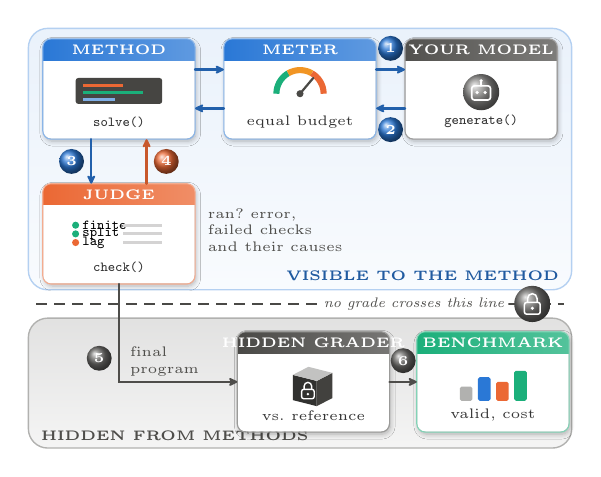
\begin{tikzpicture}[
  font=\scriptsize,
  >={Stealth[length=4pt, width=3.8pt, round]},
  flow/.style={->, line width=0.9pt, line cap=round, draw=#1},
  flow/.default=fingray!85!black,
  lab/.style={font=\tiny, text=fingray!95!black, align=center, inner sep=1pt},
  title/.style={font=\footnotesize\bfseries, anchor=south west, inner sep=0pt},
  ball/.style={circle, shading=ball, ball color=#1, text=white, font=\tiny\bfseries,
               inner sep=0pt, minimum size=9pt},
  ball/.default=finblue,
  iso/.style={x={(0.95cm,-0.24cm)}, y={(0.62cm,0.32cm)}, z={(0cm,1cm)}},
  callout/.style={align=left, anchor=west, inner sep=2.2pt, text width=2.9cm, font=\tiny,
                  text=black!85, fill=white, rounded corners=2.5pt,
                  blur shadow={shadow blur steps=6, shadow xshift=0.4pt,
                               shadow yshift=-0.8pt, shadow opacity=22}},
]
% ================================================================== (b) one episode

\def\pw{6.9}
% \card{name}{x,y}{colour}{HEADER}{illustration}{caption}
\newcommand{\card}[6]{%
  \node[fill=white, rounded corners=3pt, minimum width=1.92cm, minimum height=1.26cm,
        blur shadow={shadow blur steps=7, shadow xshift=0.5pt, shadow yshift=-1pt,
                     shadow opacity=28}] (#1) at (#2) {};
  \begin{scope}
    \clip[rounded corners=3pt] (#1.south west) rectangle (#1.north east);
    \shade[left color=#3, right color=#3!75!white] ($(#1.north west) + (0, -0.27)$) rectangle (#1.north east);
  \end{scope}
  \draw[#3!55, line width=0.4pt, rounded corners=3pt] (#1.south west) rectangle (#1.north east);
  \node[font=\tiny\bfseries, text=white, anchor=center] at ($(#1.north) + (0, -0.135)$) {#4};
  \begin{scope}[shift={($(#1.center) + (0, -0.06)$)}] #5 \end{scope}
  \node[font=\tiny, text=black!80, anchor=south] at ($(#1.south) + (0, 0.02)$) {#6};}



\shade[top color=finblue!10, bottom color=finblue!3, rounded corners=7pt, draw=finblue!35,
       line width=0.5pt] (0, 4.27) rectangle (\pw, 0.95);
\shade[top color=fingray!17, bottom color=fingray!6, rounded corners=7pt, draw=fingray!45,
       line width=0.5pt] (0, 0.59) rectangle (\pw, -1.06);
\node[lab, anchor=south east, font=\tiny\bfseries, text=finblue!75!black] at (\pw-0.12, 1.02)
  {VISIBLE TO THE METHOD};
\node[lab, anchor=south west, font=\tiny\bfseries, text=fingray!95!black] at (0.12, -1.0)
  {HIDDEN FROM METHODS};

\card{method}{1.15, 3.5}{finblue}{METHOD}{%
  \fill[fingray!85!black, rounded corners=1pt] (-0.55, -0.13) rectangle (0.55, 0.2);
  \foreach \i/\c/\l in {0/finorange/0.5, 1/finaqua/0.75, 2/finblue!60/0.4}
    \fill[\c] (-0.45, {0.12-\i*0.09}) rectangle ({-0.45+\l}, {0.085-\i*0.09});}{\texttt{solve()}}
\card{meter}{3.45, 3.5}{finblue}{METER}{%
  \foreach \a/\b/\c in {180/120/finaqua, 120/60/finorange!70!yellow, 60/0/finorange}
    \draw[\c, line width=2.2pt] (\a:0.3) arc[start angle=\a, end angle=\b, radius=0.3];
  \draw[fingray!90!black, line width=0.8pt, line cap=round] (0,0) -- (50:0.26);
  \fill[fingray!90!black] (0,0) circle (0.045);}{equal budget}
\card{llm}{5.75, 3.5}{fingray}{YOUR MODEL}{%
  \node[circle, shading=ball, ball color=fingray!65, minimum size=0.46cm] at (0, 0.02) {};
  \pic[draw=white, fill=white, line width=0.6pt] at (0, 0.02) {fin robot};}{\texttt{generate()}}
\card{judge}{1.15, 1.66}{finorange}{JUDGE}{%
  \foreach \yy/\c/\t in {0.17/finaqua/finite, 0.06/finaqua/split, -0.05/finorange/lag} {
    \fill[\c] (-0.55, \yy) circle (0.045);
    \node[font=\fontsize{4}{4}\selectfont\ttfamily, anchor=west, inner sep=0pt] at (-0.47, \yy) {\t};
    \fill[fingray!25] (0.05, {\yy-0.02}) rectangle (0.55, {\yy+0.02});}}{\texttt{check()}}
\card{grader}{3.62, -0.22}{fingray!90!black}{HIDDEN GRADER}{%
  \begin{scope}[iso, scale=0.32, shift={(-0.6, -0.4, -0.55)}]
    \fill[fingray!80!black] (1,0,0) -- (1,1,0) -- (1,1,1) -- (1,0,1) -- cycle;
    \fill[fingray!60!black] (0,0,0) -- (1,0,0) -- (1,0,1) -- (0,0,1) -- cycle;
    \fill[fingray!35] (0,0,1) -- (1,0,1) -- (1,1,1) -- (0,1,1) -- cycle;
  \end{scope}
  \pic[draw=white, fill=white, line width=0.5pt, scale=0.8] at (-0.07, -0.05) {fin lock};}{vs.\ reference}
\card{report}{5.9, -0.22}{finaqua}{BENCHMARK}{%
  \foreach \i/\h/\c in {0/0.18/fingray!45, 1/0.30/finblue, 2/0.24/finorange, 3/0.38/finaqua}
    \fill[\c, rounded corners=0.6pt] ({-0.42+\i*0.23}, -0.18) rectangle ({-0.26+\i*0.23}, {-0.18+\h});}{valid, cost}

% the barrier
\draw[fingray!90!black, line width=1pt, dash pattern=on 4pt off 2.5pt] (0.1, 0.77) -- (\pw-0.1, 0.77);
\node[ball=fingray!80, minimum size=0.46cm] (barrier) at (\pw - 0.5, 0.77) {};
\pic[draw=white, fill=white, line width=0.55pt] at (barrier) {fin lock};
\node[lab, anchor=east, font=\tiny\itshape, fill=white, rounded corners=1.5pt, inner sep=1.5pt]
  at ($(barrier.west) + (-0.06, 0)$) {no grade crosses this line};

% arrows and steps
\draw[flow=finblue!80!black] ([yshift=7pt]method.east) -- ([yshift=7pt]meter.west);
\draw[flow=finblue!80!black] ([yshift=7pt]meter.east) -- ([yshift=7pt]llm.west);
\draw[flow=finblue!80!black] ([yshift=-7pt]llm.west) -- ([yshift=-7pt]meter.east);
\draw[flow=finblue!80!black] ([yshift=-7pt]meter.west) -- ([yshift=-7pt]method.east);
\node[ball] at ($([yshift=7pt]meter.east)!0.5!([yshift=7pt]llm.west) + (0, 0.27)$) {1};
\node[ball] at ($([yshift=-7pt]llm.west)!0.5!([yshift=-7pt]meter.east) + (0, -0.27)$) {2};
\draw[flow=finblue!80!black] ([xshift=-10pt]method.south) -- ([xshift=-10pt]judge.north);
\draw[flow=finorange!85!black] ([xshift=10pt]judge.north) -- ([xshift=10pt]method.south);
\node[ball] at ($([xshift=-10pt]method.south)!0.5!([xshift=-10pt]judge.north) + (-0.25, 0)$) {3};
\node[ball=finorange] at ($([xshift=10pt]judge.north)!0.5!([xshift=10pt]method.south) + (0.25, 0)$) {4};
\node[lab, anchor=west, align=left] at ($(judge.east) + (0.12, 0.05)$)
  {ran?\ error,\\failed checks\\and their causes};
\draw[flow=fingray!95!black] (judge.south) |- (grader.west);
\node[ball=fingray!85] at ($(judge.south |- grader.west) + (-0.25, 0.3)$) {5};
\node[lab, anchor=south west, align=left] at ($(judge.south |- grader.west) + (0.1, 0.03)$)
  {final\\program};
\draw[flow=fingray!95!black] (grader.east) -- (report.west);
\node[ball=fingray!85] at ($(grader.east)!0.5!(report.west) + (0, 0.27)$) {6};


\end{tikzpicture}

\caption{One episode. (1)~Each prompt and (2)~each program pass through the meter; (3)~the
method sends code to the judge and (4)~sees only what \texttt{check()} returns. (5)~After
\texttt{solve()} returns, the hidden grader runs on the final program, and (6)~its verdict
goes only to the benchmark report.}
\label{fig:episode}
\end{figure}

\paragraph{What a method sees.}
\texttt{solve()} gets the task text and a judge on which it can only call
\texttt{check(code)}. That returns whether the program ran, its error, each check's result
and the causes of the failed ones, never the grade (Figure~\ref{fig:episode}). Learning
methods may use development grades to keep or reject a candidate, but no text a model reads
contains a grade.

\paragraph{Equal budgets.}
A meter refuses any call beyond the budget and records which limit stopped the episode.
Each episode gets \BudgetAttempts{} program executions, \BudgetCalls{} model calls
(reflections and reviews included) and \BudgetTokens{} generated tokens. Learning methods
also get \FitEpisodes{} development episodes, \FitProposals{} proposals, \FitCalls{} calls
and \FitTokens{} tokens.

\paragraph{Methods.}
The \NMethods{} methods (Appendix Table~\ref{tab:methods}) keep the mechanism each is known
for: \texttt{NoImprove} (one program); \texttt{SelfDebug}, which returns only errors
\citep{chen2024selfdebug}; \texttt{CheckFeedback}, which returns the failed checks with
causes and cards; \texttt{Reflexion}, which adds a written reflection before each retry
\citep{shinn2023reflexion}; \texttt{Team}, with one reviewer per rule family;
\texttt{Evolve}, which evolves a prompt addendum on development tasks
\citep{agrawal2026gepa}; and \texttt{PlaybookLearning}
\citep{zhao2024expel,suzgun2026dynamic}. The playbook proposer sees development traces
without grades, and one proposal edits one entry. A candidate is accepted only if its score
does not drop on either of two disjoint halves of the development tasks, rises on one, and
no task that passed every check before now fails one (the \emph{no-regression} rule;
Appendix Figure~\ref{fig:gate}).

\paragraph{Skill arms.}
Two switches split the skills: \texttt{cards} adds the task's rule cards to the prompt and
the feedback; \texttt{library} adds the interface text and allows
\texttt{import fin\_skills}. Their \NArms{} combinations (\texttt{none}, \texttt{cards},
\texttt{library}, \texttt{cards+library}) all keep the task definition and see the failed
checks with their causes. Within an arm, \texttt{NoImprove} versus \texttt{CheckFeedback}
measures the checks and \texttt{CheckFeedback} versus \texttt{PlaybookLearning} measures
self-improvement; for one method, comparing arms measures the skills (Appendix
Figure~\ref{fig:arms}).

\section{Task suite}
\label{sec:tasks}

\NTasks{} tasks cover \NTaskAlgorithms{} algorithms in \NFamilies{} families, two variants
each (Appendix Table~\ref{tab:tasks}). A task states a rule in prose; the model implements
\texttt{solve(prices, split\_factors)} returning positions, or for volatility, risk and
forecast tasks the value known at the previous close. Each task can be solved by hand or by
one library call. The rules are the momentum, volatility-scaling and allocation baselines
that learned strategies are measured against
\citep{lim2019enhancing,wood2022slow,zhang2020deep}.

\paragraph{Data.}
Synthetic panels have four assets and \NRows{} business days of seeded Gaussian returns,
with four splits at fixed rows (2-for-1, 3-for-1, 3-for-2, 1-for-2), on \NSeeds{} seeds.
Variant~a gives cumulative factors in alphabetical order; variant~b gives event ratios,
shuffled columns and other parameters. The suite also has a real panel: as-traded
closes of Amazon, Shopify, Alphabet and Tesla for \NRealRows{} sessions from \RealFirst{} to
\RealLast{}, in which all four split (20-, 10-, 20- and 3-for-1; Appendix
Figure~\ref{fig:real}). Yahoo Finance serves the
closes split-adjusted; we rebuild as-traded quotes from a split table checked against the
companies' announcements and published pre-split closes, and release the fetch code and the
file's SHA-256, since the prices may not be redistributed.

\paragraph{Judge and hidden grader.}
The judge runs each program in a separate process with a memory limit and a 120-second
timeout (in our runs also confined with Landlock and seccomp), refuses \texttt{import fin\_skills} without library access, and applies the three
checks of \S\ref{sec:library}. A program is \emph{valid} only if it
ran, passed every check and matches an independent numpy reference within $10^{-8}$
($10^{-5}$ for \texttt{min\_variance}). A program that passes the checks but is wrong is
\emph{accepted but wrong}; we report that rate because the checks cannot see it.

\paragraph{Qualification.}
Before any model ran: on every task and data panel, the reference agrees with the library
to within $\RefGapOther$ ($\RefGapMinVariance$ for \texttt{min\_variance}); a correct
program passes every check and is graded valid; and on a position task and a table task,
planted versions of each failure (same close, no adjustment, factors cumulated twice,
missing warm-up) fail their check and the grade. Building the references exposed a library
defect: the long-only minimum-variance optimiser stopped early on daily-scale covariances,
off by up to $1.2\times10^{-2}$, until we rescaled the covariance before solving.

\paragraph{Split.}
The split is by algorithm. The \NForcedDev{} algorithms a model has already seen go to
development, and a seeded draw sends \NDrawnDev{} of the other \NDrawn{} there too:
\NDevTasks{} development and \NHeldTasks{} held-out tasks, the latter covering all
\NFamilies{} families.

\section{Study protocol}
\label{sec:study}

We fixed the tasks, prompts, seeds, budgets, models and contrasts before any test run, on
the suite as it stood on 8~November 2026: \StudyDevTasks{} development and
\StudyHeldTasks{} held-out position tasks on synthetic panels (Bollinger, RSI and Donchian
rules, two variants each). The tasks added since, and the real panel, are not part of the
study. It has three tracks.

\paragraph{P: feedback and library.}
The three controlled arms, with and without the library, on the \StudyHeldTasks{} held-out
tasks and \StudySeeds{} seeds: \StudyPEpisodes{} episodes per model. Three contrasts were
declared: \texttt{Check} against \texttt{Repeat} and \texttt{Explain} against
\texttt{Check}, both without the library, and library against none under \texttt{Explain}.

\paragraph{E: external questions.}
\StudyEQuestions{} public questions from the two table-and-text program-synthesis tasks of
BizBench \citep{krumdick2024bizbench} (\StudyECodeFinQA{} CodeFinQA, \StudyECodeTATQA{}
CodeTAT-QA), selected by a rule fixed before any model output: a numeric answer, a prompt
that fits every core model's context, no duplicate in the training split, one question per
group of shared context. The model writes one program per question, with and without the
library and without feedback: \StudyEEpisodes{} episodes per model. An answer counts if the
program runs and returns the public label exactly; BizBench scores within 1\%, which we report as
a sensitivity analysis.

\paragraph{S: seven methods.}
The \NMethods{} methods of \S\ref{sec:methods}, with and without the library, on the same
tasks and seeds, for \StudyCoreModels{} core models: \StudySEpisodes{} episodes and
\StudySFits{} fits on the development tasks.

\paragraph{Models and analysis.}
Tracks P and E run on \StudyModels{} open-weight instruction models from \StudyFamilies{}
families, 2B to 32B parameters, in BF16 at temperature 0.1, with a \StudyContext{}-token
context (16,384 for one model with a smaller native limit) and at most \StudyOutputCap{}
generated tokens per call. Every refusal, truncated reply and failed program stays in the
denominator. The position tasks cover only \StudyAlgorithms{} algorithms, and variants and
seeds are not independent of them: with three clusters a sign-flip test cannot go below
$p=0.25$. We therefore report P and S as effects per algorithm, without significance
claims. Track E weights its two sources equally.

\section{Preliminary results}
\label{sec:results}

\pending{Per track and model, for the models whose runs finished: valid rate by arm (P),
by library condition (E) and by method (S), each with the accepted-but-wrong rate, the share
of replies with no program, and the cost in calls and tokens; the three P contrasts per
algorithm. Models still running are listed as incomplete, not averaged in.}

\paragraph{Limitations.}
The study covers three position algorithms on synthetic panels and one set of public
questions; the newer tasks, the real panel and the rule-card switch are released but not
evaluated here. All tasks are public, so a model may have seen them. The checks reject only
the failures they were written for, hence the accepted-but-wrong rate. In the frozen source,
\texttt{Evolve} chose the development failures it showed its proposer by the hidden grade;
the release fixes this, and the \texttt{Evolve} runs reported here predate the fix. All
models are open-weight, under one attempt budget.


\bibliography{../latex_acl2027/references}

\appendix
\section{Self-improvement methods}
\label{app:methods}

\begin{table*}[h]
\centering
\small
\setlength{\tabcolsep}{4pt}
\begin{tabular}{@{}lp{5.3cm}p{3.9cm}p{2.8cm}@{}}
\toprule
Method & At test time & Learned on development tasks & In the spirit of \\
\midrule
\texttt{NoImprove} & one program, no feedback & -- & baseline \\
\texttt{SelfDebug} & retry with the error only; stop once the program runs & -- &
\citet{chen2024selfdebug} \\
\texttt{CheckFeedback} & retry with the failed checks, their causes and cards & -- &
verifier feedback \\
\texttt{Reflexion} & as \texttt{CheckFeedback}, plus a written reflection before each retry &
-- & \citet{shinn2023reflexion} \\
\texttt{PlaybookLearning} & as \texttt{CheckFeedback}, with a frozen playbook in the prompt &
playbook entries, through the gated loop & \citet{zhao2024expel,suzgun2026dynamic} \\
\texttt{Team} & a writer and one reviewer per rule family, from the same model & -- &
multi-role review \\
\texttt{Evolve} & as \texttt{CheckFeedback}, with an evolved prompt addendum & the addendum,
over \EvolveGenerations{} generations on \EvolveMinibatch{} tasks & \citet{agrawal2026gepa} \\
\bottomrule
\end{tabular}
\caption{The \NMethods{} self-improvement methods. All share the prompt, the judge and the
budget; each keeps the mechanism it is known for. They are not reproductions of the original
systems.}
\label{tab:methods}
\end{table*}

\texttt{Reflexion} asks for a reflection of at most five sentences, without code, and keeps
the reflections for the rest of the episode. In \texttt{Team}, a reviewer is asked only when a
check of its own family failed; it sees the program, the failed checks, their causes and its
family's cards, and answers with a diagnosis rather than code. \texttt{Evolve} rewrites a
prompt addendum of at most 1,200 characters from the visible failures of the current best
addendum, and keeps a candidate only if it scores strictly higher on the same development
tasks. The playbook is a list of short entries on three surfaces (tool usage, retrieval,
experience). Its loop rejects whitespace-only and repeated edits, and appends every proposal,
evaluation and decision to a journal whose receipts carry evidence hashes; a frozen playbook
cannot change. A stricter \emph{all-pass} rule, which vetoes any candidate while a single
task fails, blocks learning for a weak model, so we use no-regression.

\begin{figure*}[t]
\centering
\resizebox{\textwidth}{!}{% Figure: the gated playbook loop of PlaybookLearning, told in pictures. The halves are the
% development and validation splits of the development tasks (split by algorithm), and the gate is
% guard_rule="no_regression" in fin_skills/rsi/core.py: accept only if neither half scores lower,
% one scores higher and no task that passed its checks now fails. The dots are an example, not
% results. The proposal budget is a macro from numbers.tex.
\InputIfFileExists{figures/glyphs}{}{% Glyphs for the method figures (episode, gate, arms). Pictures first, words only as labels.%
% Colours, text styles, lines, corners, shadows and arrows come from figures/figstyle.tex,%
% icons from figures/lucide.tex. Load figstyle if the document has not.%
\ifcsname figTitleFont\endcsname\else\InputIfFileExists{figures/figstyle}{}{\input{../latex_acl2027/figures/figstyle}}\fi%
% \gpage{centre}{w}{h}{fill}: a page with a folded corner.%
\providecommand{\gpage}[4]{%
  \begin{scope}[shift={#1}]%
    \path[fill=#4, draw=gline, line width=0.5pt, line join=round, gshade]%
      ({-#2/2},{-#3/2}) -- ({#2/2},{-#3/2}) -- ({#2/2},{#3/2-0.2}) -- ({#2/2-0.2},{#3/2}) -- ({-#2/2},{#3/2}) -- cycle;%
    \draw[gline, line width=0.5pt, line join=round, fill=gline!40] ({#2/2-0.2},{#3/2}) -- ({#2/2-0.2},{#3/2-0.2}) -- ({#2/2},{#3/2-0.2});%
  \end{scope}}%
% \gbar{x0}{y}{length}{colour}: one line of text or code, drawn as a rounded bar.%
\providecommand{\gbar}[4]{\draw[#4, line width=2.4pt, line cap=round] (#1,#2) -- ({#1+#3},#2);}%
% \gcheck{centre}{state}: a check that passed (1) or failed (0), Lucide check or x on a disc.%
\providecommand{\gcheck}[2]{%
  \ifnum#2=1 \fill[figok] #1 circle (0.13);%
    \pic[draw=white, line width=0.85pt, scale=0.62] at #1 {lu check};%
  \else \fill[figbad] #1 circle (0.13);%
    \pic[draw=white, line width=0.85pt, scale=0.62] at #1 {lu x};\fi}%
% \gcard{centre}: a rule card, small and blue.%
\providecommand{\gcard}[1]{%
  \begin{scope}[shift={#1}]%
    \path[fill=finblue!12, draw=finblue!70, line width=0.55pt, fig item, gshade] (-0.22,-0.16) rectangle (0.22,0.16);%
    \draw[finblue!70, line width=0.9pt, line cap=round] (-0.13,0.05) -- (0.13,0.05) (-0.13,-0.05) -- (0.06,-0.05);%
  \end{scope}}%
% \glock{centre}: a padlock (Lucide lock) on a white disc, so it can sit on a line.%
\providecommand{\glock}[1]{%
  \fill[white] #1 circle (0.19);%
  \pic[draw=figink!80, line width=0.95pt, scale=1.05] at #1 {lu lock};}%
% \gbot{centre}{radius}: the model, a dark disc with the Lucide bot icon.%
\providecommand{\gbot}[2]{%
  \path[fill=figink, fig shadow] #1 circle (#2);%
  \pic[draw=white, line width=0.75pt, scale={4.2*#2}] at #1 {lu bot};}%
}%
\begin{tikzpicture}[x=1cm, y=1cm, font=\sffamily]
\def\Y{1.35}
\def\book#1#2{% \book{centre x}{colour of the new entry, or n for none}
  \gpage{(#1+0.1,\Y+0.08)}{1.0}{1.2}{white}
  \gpage{(#1,\Y)}{1.0}{1.2}{white}
  \foreach \k/\l in {1/0.62, 2/0.5, 3/0.66} {\gbar{#1-0.36}{\Y+0.36-0.18*\k}{\l}{gline}}
  \ifx#2n\else\gbar{#1-0.36}{\Y+0.36-0.18*4}{0.56}{#2}\fi}
\def\tasks#1#2#3{% \tasks{x}{y}{how many of 4 passed}
  \foreach \i in {1,...,4} {
    \ifnum\i>#3 \draw[gmid!70, line width=0.5pt] ({#1+0.2*(\i-1)},#2) circle (0.062);
    \else \fill[gok] ({#1+0.2*(\i-1)},#2) circle (0.068);\fi}}
% ---------------------------------------------------------------- playbook, proposer, candidate
\book{1.05}{n}
\node[gword] at (1.05,\Y-0.88) {playbook P};
\node[gnote] at (1.05,\Y-1.15) {in every prompt};
\draw[gflow] (1.72,\Y) -- (3.15,\Y);
\gbot{(3.65,\Y)}{0.33}
\node[gword] at (3.65,\Y-0.88) {proposer};
\node[gnote] at (3.65,\Y-1.15) {sees checks, not grades};
\draw[gflow] (4.1,\Y) -- (5.55,\Y);
\book{6.25}{gok}
\node[gword] at (6.25,\Y-0.88) {candidate P$'$};
\node[gnote] at (6.25,\Y-1.15) {one entry added};
\draw[gflow] (6.92,\Y) -- (7.5,\Y);
% ---------------------------------------------------------------- two halves
\begin{scope}[shift={(7.62,0)}]
  \path[fill=white, draw=gline, line width=0.5pt, rounded corners=2pt, gshade] (0,\Y-0.62) rectangle (3.3,\Y+0.62);
  \draw[gline, line width=0.5pt] (1.73,\Y-0.5) -- (1.73,\Y+0.5);
  \node[gnote, anchor=east] at (0.34,\Y+0.2) {P};
  \node[gnote, anchor=east] at (0.34,\Y-0.2) {P$'$};
  \tasks{0.5}{\Y+0.2}{3} \tasks{0.5}{\Y-0.2}{3}
  \tasks{2.05}{\Y+0.2}{2} \tasks{2.05}{\Y-0.2}{3}
  \node[gword] at (0.86,\Y-0.88) {development};
  \node[gword] at (2.42,\Y-0.88) {validation};
  \node[gnote] at (0.86,\Y-1.15) {same};
  \node[gnote] at (2.42,\Y-1.15) {higher};
\end{scope}
\draw[gflow] (10.98,\Y) -- (11.88,\Y);
% ---------------------------------------------------------------- the gate
\path[fill=white, draw=gink, line width=0.7pt, gshade] (12.45,\Y+0.5) -- (12.97,\Y) -- (12.45,\Y-0.5) -- (11.93,\Y) -- cycle;
\gcheck{(12.45,\Y)}{1}
\node[gword] at (12.45,\Y-0.88) {no-regression gate};
\node[gnote] at (12.45,\Y-1.15) {no half lower, one higher};
% accept: P' becomes the playbook
\draw[-{Latex[length=1.7mm,width=1.4mm]}, gok, line width=0.9pt] (12.45,\Y+0.52) .. controls (12.45,\Y+1.6) and (1.05,\Y+1.6) .. (1.05,\Y+0.74);
\node[gnote, fill=white, inner sep=1pt, text=gok!80!black] at (6.75,\Y+1.33) {accept: P$'$ becomes P};
% reject: P stays
\draw[-{Latex[length=1.7mm,width=1.4mm]}, gbad!80, line width=0.9pt] (12.99,\Y) -- (14.42,\Y);
\begin{scope}[opacity=0.55]\book{15.1}{gok}\end{scope}
\draw[gbad, line width=1.2pt, line cap=round] (14.75,\Y-0.4) -- (15.45,\Y+0.4) (14.75,\Y+0.4) -- (15.45,\Y-0.4);
\node[gword] at (15.1,\Y-0.88) {reject};
\node[gnote] at (15.1,\Y-1.15) {P stays};
\node[gnote, anchor=east] at (15.95,\Y+1.05) {at most \FitProposals{} proposals};
\end{tikzpicture}
}
\caption{The gated playbook loop of \texttt{PlaybookLearning}. The proposer reads development
traces without grades and adds one entry; the current and the candidate playbook are scored on
two disjoint halves of the development tasks (dots: tasks that passed their checks; an example,
not results). The no-regression gate accepts the candidate only if neither half is lower, one is
higher and no task that passed before now fails.}
\label{fig:gate}
\end{figure*}

\section{Experiment design}
\label{app:design}

\begin{figure}[h]
\centering
% Figure: the skill arms (rsi.ARMS) and the method contrasts of the component ablation, in
% pictures. A blue card stands for the rule cards and a dark square for the library interface;
% faint means the arm leaves it out. Bold frames are the arms of the main comparison.
\InputIfFileExists{figures/glyphs}{}{% Glyphs for the method figures (episode, gate, arms). Pictures first, words only as labels.%
% Colours, text styles, lines, corners, shadows and arrows come from figures/figstyle.tex,%
% icons from figures/lucide.tex. Load figstyle if the document has not.%
\ifcsname figTitleFont\endcsname\else\InputIfFileExists{figures/figstyle}{}{\input{../latex_acl2027/figures/figstyle}}\fi%
% \gpage{centre}{w}{h}{fill}: a page with a folded corner.%
\providecommand{\gpage}[4]{%
  \begin{scope}[shift={#1}]%
    \path[fill=#4, draw=gline, line width=0.5pt, line join=round, gshade]%
      ({-#2/2},{-#3/2}) -- ({#2/2},{-#3/2}) -- ({#2/2},{#3/2-0.2}) -- ({#2/2-0.2},{#3/2}) -- ({-#2/2},{#3/2}) -- cycle;%
    \draw[gline, line width=0.5pt, line join=round, fill=gline!40] ({#2/2-0.2},{#3/2}) -- ({#2/2-0.2},{#3/2-0.2}) -- ({#2/2},{#3/2-0.2});%
  \end{scope}}%
% \gbar{x0}{y}{length}{colour}: one line of text or code, drawn as a rounded bar.%
\providecommand{\gbar}[4]{\draw[#4, line width=2.4pt, line cap=round] (#1,#2) -- ({#1+#3},#2);}%
% \gcheck{centre}{state}: a check that passed (1) or failed (0), Lucide check or x on a disc.%
\providecommand{\gcheck}[2]{%
  \ifnum#2=1 \fill[figok] #1 circle (0.13);%
    \pic[draw=white, line width=0.85pt, scale=0.62] at #1 {lu check};%
  \else \fill[figbad] #1 circle (0.13);%
    \pic[draw=white, line width=0.85pt, scale=0.62] at #1 {lu x};\fi}%
% \gcard{centre}: a rule card, small and blue.%
\providecommand{\gcard}[1]{%
  \begin{scope}[shift={#1}]%
    \path[fill=finblue!12, draw=finblue!70, line width=0.55pt, fig item, gshade] (-0.22,-0.16) rectangle (0.22,0.16);%
    \draw[finblue!70, line width=0.9pt, line cap=round] (-0.13,0.05) -- (0.13,0.05) (-0.13,-0.05) -- (0.06,-0.05);%
  \end{scope}}%
% \glock{centre}: a padlock (Lucide lock) on a white disc, so it can sit on a line.%
\providecommand{\glock}[1]{%
  \fill[white] #1 circle (0.19);%
  \pic[draw=figink!80, line width=0.95pt, scale=1.05] at #1 {lu lock};}%
% \gbot{centre}{radius}: the model, a dark disc with the Lucide bot icon.%
\providecommand{\gbot}[2]{%
  \path[fill=figink, fig shadow] #1 circle (#2);%
  \pic[draw=white, line width=0.75pt, scale={4.2*#2}] at #1 {lu bot};}%
}%
\begin{tikzpicture}[x=1cm, y=1cm, font=\sffamily]
\def\lib#1#2{% \lib{centre}{on 1 / off 0}: the library, a code square
  \begin{scope}[shift={#1}]
    \ifnum#2=1 \path[fill=gink, rounded corners=1.5pt, gshade] (-0.2,-0.2) rectangle (0.2,0.2);
      \pic[draw=white, line width=0.6pt, scale=0.72] at (0,0) {lu code};
    \else \draw[gline, line width=0.6pt, dash pattern=on 1.5pt off 1pt, rounded corners=1.5pt] (-0.2,-0.2) rectangle (0.2,0.2);\fi
  \end{scope}}
\def\crd#1#2{% \crd{centre}{on 1 / off 0}: the rule cards
  \ifnum#2=1 \gcard{#1}\else
  \begin{scope}[shift={#1}]\draw[gline, line width=0.6pt, dash pattern=on 1.5pt off 1pt, rounded corners=1pt] (-0.22,-0.16) rectangle (0.22,0.16);\end{scope}\fi}
\def\arm#1#2#3#4#5{% \arm{x}{y}{cards}{library}{main 1/0}
  \ifnum#5=1 \path[fill=white, draw=gink, line width=0.9pt, rounded corners=2pt, gshade] ({#1-0.75},{#2-0.36}) rectangle ({#1+0.75},{#2+0.36});
  \else \path[fill=white, draw=gline, line width=0.5pt, rounded corners=2pt, gshade] ({#1-0.75},{#2-0.36}) rectangle ({#1+0.75},{#2+0.36});\fi
  \crd{({#1-0.3},#2)}{#3} \lib{({#1+0.32},#2)}{#4}}
\tikzset{both/.style={gflow, {Latex[length=1.6mm,width=1.4mm]}-{Latex[length=1.6mm,width=1.4mm]}}}
% ---------------------------------------------------------------- (a) skill arms
\node[gword, anchor=west, font=\sffamily\glab\bfseries] at (0,3.85) {(a) Skill arms};
\node[gnote] at (2.6,3.48) {no library}; \node[gnote] at (5.0,3.48) {library};
\node[gnote, anchor=east] at (1.7,2.95) {no cards}; \node[gnote, anchor=east] at (1.7,1.75) {rule cards};
\arm{2.6}{2.95}{0}{0}{0} \arm{5.0}{2.95}{0}{1}{0}
\arm{2.6}{1.75}{1}{0}{1} \arm{5.0}{1.75}{1}{1}{1}
\draw[both] (3.4,2.95) -- (4.2,2.95);
\draw[both] (3.4,1.75) -- (4.2,1.75);
\draw[both] (2.6,2.55) -- (2.6,2.15);
\draw[both] (5.0,2.55) -- (5.0,2.15);
\draw[gink, line width=0.9pt, rounded corners=1pt] (4.42,3.78) rectangle ++(0.16,0.14);
\node[gnote, anchor=west] at (4.66,3.85) {main comparison};
% ---------------------------------------------------------------- (b) method contrasts
\node[gword, anchor=west, font=\sffamily\glab\bfseries] at (0,0.95) {(b) Within one arm};
\begin{scope}[shift={(0.9,0.05)}]
  \gpage{(0,0)}{0.5}{0.62}{white}
\end{scope}
\node[gword, font=\figCodeFont] at (0.9,-0.55) {NoImprove};
\node[gnote] at (0.9,-0.8) {one program};
\begin{scope}[shift={(3.65,0.05)}]
  \gpage{(0,0)}{0.5}{0.62}{white}
  \draw[-{Latex[length=1.4mm,width=1.2mm]}, gbad!75, line width=0.8pt, dash pattern=on 2pt off 1.3pt] (0.3,0.12) .. controls (0.75,0.55) and (-0.75,0.55) .. (-0.3,0.12);
  \gcheck{(0.46,-0.18)}{0}
\end{scope}
\node[gword, font=\figCodeFont] at (3.65,-0.55) {CheckFeedback};
\node[gnote] at (3.65,-0.8) {retries on failed checks};
\begin{scope}[shift={(6.33,0.05)}]
  \gpage{(0.08,0.05)}{0.5}{0.62}{white}
  \gpage{(0,0)}{0.5}{0.62}{white}
  \gbar{-0.15}{-0.12}{0.3}{gok}
  \draw[-{Latex[length=1.4mm,width=1.2mm]}, gbad!75, line width=0.8pt, dash pattern=on 2pt off 1.3pt] (0.3,0.12) .. controls (0.75,0.55) and (-0.75,0.55) .. (-0.3,0.12);
\end{scope}
\node[gword, font=\figCodeFont] at (6.33,-0.55) {PlaybookLearning};
\node[gnote] at (6.33,-0.8) {and keeps a playbook};
\draw[gflow] (1.45,0.05) -- (3.1,0.05);
\draw[gflow] (4.2,0.05) -- (5.8,0.05);
\node[gnote] at (2.27,0.66) {+ checks};
\node[gnote] at (5.0,0.66) {+ self-improvement};
\end{tikzpicture}

\caption{(a) The four skill arms: a blue card for the rule cards, a dark square for the library
interface, a dashed outline for what an arm leaves out. Bold frames are the arms of the main
comparison; arrows join arms that differ in one component. (b) Within one arm,
\texttt{NoImprove} versus \texttt{CheckFeedback} measures the checks and \texttt{CheckFeedback}
versus \texttt{PlaybookLearning} measures self-improvement.}
\label{fig:arms}
\end{figure}

\section{Real-price panel}
\label{app:real}

\begin{figure*}[h]
\centering
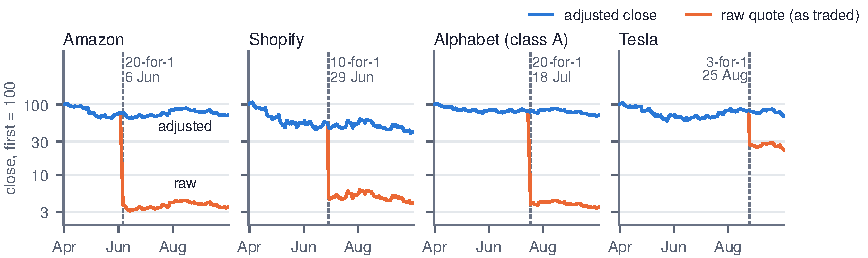
\includegraphics[width=\textwidth]{figures/real_panel}
\caption{The real-price panel: raw quotes (as traded) and adjusted closes of the four stocks,
each indexed to 100 at the first close, on a log scale. Every stock splits inside the window;
a program that ignores the split factors sees a one-day loss of 67\% to 95\%.}
\label{fig:real}
\end{figure*}

\section{Rule cards}
\label{app:cards}

\begin{table}[h]
\centering
\scriptsize
\input{cards_table}
\caption{Rule cards by family, the checks that verify each one, and whether the card names a
library call that follows the rule.}
\label{tab:cards}
\end{table}

\section{Task suite}
\label{app:tasks}

\begin{table}[h]
\centering
\footnotesize
\input{tasks_table}
\caption{The \NTaskAlgorithms{} algorithms of the task suite, with their split and the
one-step library call that solves them. Each algorithm has two tasks (variants a and b).}
\label{tab:tasks}
\end{table}


\end{document}
